\documentclass[11pt]{article}

%% Packages
\usepackage{fontspec}

\setmainfont{Times New Roman}

\usepackage[margin=1in]{geometry}

\AtBeginDocument{\fontsize{11pt}{14pt}\selectfont}

\setlength{\parindent}{0.63cm}

\setlength{\parskip}{0pt}

\usepackage{tikz}

\usetikzlibrary{positioning,arrows.meta}
\usepackage{amsmath,amssymb,amsthm}
\usepackage{mathtools}
\usepackage{graphicx}
\usepackage{booktabs}
\usepackage{hyperref}



\usepackage{comment}

\usepackage[
  authordate,
  backend=biber,
  maxcitenames=2,
  mincitenames=1,
  maxbibnames=6,
  minbibnames=3,
  doi=true,
  url=true,
  isbn=false
]{biblatex-chicago}

\addbibresource{references.bib}

% Do not print Zotero access dates
\AtEveryBibitem{%
  \clearfield{urlyear}%
  \clearfield{urlmonth}%
  \clearfield{urlday}%
}

% Prefer DOI over an ordinary URL when both are available
\renewbibmacro*{doi+eprint+url}{%
  \printfield{doi}%
  \newunit\newblock
  \iffieldundef{doi}
    {\usebibmacro{eprint}%
     \newunit\newblock
     \usebibmacro{url+urldate}}
    {}%
}


%%%%%%%%%%%%%%%%%%%%%%%%%%%%%%%%%%%%%%%%%%%%%%%%%%%%%%%%%%%%%%%%%%%%%%%%%%%%%%

\begin{document}


%%%%%%%%%%%%%%%%%%%%%%%%%%%%%%%%%%%%%%%%%%%%%%%%%%%%%%%%%%%%%%%%%%%%%%%%%%%%%%
%% Title Page (Not Numbered)
%%%%%%%%%%%%%%%%%%%%%%%%%%%%%%%%%%%%%%%%%%%%%%%%%%%%%%%%%%%%%%%%%%%%%%%%%%%%%%

\begin{titlepage}

\thispagestyle{empty}

\begin{center}

{\Large\bfseries
From Population Knowledge to Patient Reasoning:\\[0.3em]
Instantiation and Dynamic Clinical Inquiry
}

\vspace{1.5cm}

{\large Sean M. Collins, PT, ScD}

\vspace{0.5cm}

Professor of Physical Therapy\\
School of Health\\
Plymouth State University\\
Plymouth, NH, USA

\vspace{0.5cm}

Email: smcollins1@plymouth.edu

\end{center}


\noindent


\end{titlepage}

\clearpage

\setcounter{page}{1}

\begin{center}

{\Large\bfseries
From Population Knowledge to Patient Reasoning:\\[0.3em]
Instantiation and Dynamic Clinical Inquiry
}

\vspace{1cm}


\end{center}

\vspace{0.5em}

\begin{abstract}
Clinical reasoning requires a patient-specific representation that supports explanation, prediction, intervention, and continued inquiry. Scientific knowledge, however, is expressed at the level of classes rather than patients. This paper identifies the transformation from generalized causal knowledge and patient-specific evidence into an individualized explanatory representation as clinical instantiation. The instantiated causal model represents the clinician’s provisional, fallible understanding of which mechanisms may be operative in a patient at a particular time. This framework clarifies how population knowledge becomes patient-specific reasoning, complements existing approaches to clinical inference, and provides a conceptual basis for personalized medicine, education, causal modeling, and intelligent clinical systems.

\vspace{0.5em}
\noindent\textit{Keywords:} causal models; knowledge representation; personalized medicine; mechanistic reasoning; evidence-based practice
\end{abstract}

%%%%%%%%%%%%%%%%%%%%%%%%%%%%%%%%%%%%%%%%%%%%%%%%%%%%%%%%%%%%%%%%%%%%%%%%%%%%%%

\newpage

%%%%%%%%%%%%%%%%%%%%%%%%%%%%%%%%%%%%%%%%%%%%%%%%%%%%%%%%%%%%%%%%%%%%%%%%%%%%%%
\section{Introduction}

Clinical reasoning depends upon a patient-specific representation capable of supporting explanation, prediction, and intervention. Scientific research develops knowledge concerning causal mechanisms, associations, interventions, and disease processes across populations. Clinical practice, however, is concerned with particular patients, each presenting with unique histories, physiologic characteristics, environmental influences, and evolving clinical circumstances. The central intellectual challenge of clinical practice is constructing a representation of an individual patient through which scientific knowledge can inform rational action.

This has been identified as the core challenge of clinical inquiry
\parencite{collins_dynamic_2014, collins_synthesis_2018, anjum2020rethinking}.
Although research produces increasingly sophisticated knowledge concerning disease mechanisms, diagnostic tests, and therapeutic interventions, clinicians must continually determine what is relevant to the patient before them. Randomized trials estimate average treatment effects. Mechanistic investigations identify causal relationships. Observational studies characterize associations among variables. None of these directly answers the clinician's immediate question:
\emph{What is occurring in this patient, and what should be done next?}
Between scientific knowledge and clinical action lies a representational process that remains incompletely understood.

Numerous theories illuminate important aspects of this process.
Bayesian reasoning provides a normative framework for updating beliefs under uncertainty.
Structural causal models provide formal representations for causal relationships, interventions, and counterfactual reasoning once an appropriate causal model has been specified \parencite{pearl_causality_2013}. Hypothetico-deductive models emphasize iterative hypothesis generation and testing, while pattern recognition and illness-script theories describe the role of experience in rapid clinical judgment. Decision theory explains rational action under uncertainty, and research on expertise highlights the adaptive strategies employed by experienced clinicians. Collectively, these approaches have substantially advanced understanding of clinical reasoning. Nevertheless, they primarily describe how clinicians update beliefs, generate hypotheses, recognize patterns, or make decisions once a patient-specific representation is available. They say comparatively little about the prior representational problem considered here: how population-derived causal knowledge and evidence concerning a particular patient jointly determine the patient-specific representation within which such inferential operations subsequently occur.

The distinction is important. Scientific knowledge is inherently general. It represents current understanding of mechanisms, relationships, and interventions in populations
\parencite{collins_synthesis_2018}.
Clinical reasoning, by contrast, concerns a single individual during an evolving clinical encounter. The clinician must determine which mechanisms are operative in this patient, how those mechanisms interact, which interventions are most likely to modify them, and how subsequent observations should alter future reasoning. Population knowledge must therefore undergo a representational transformation before it can guide rational action in an individual case \parencite{collins_dynamic_2014}.
Despite its centrality to clinical practice, this transformation has received comparatively little explicit philosophical attention, even as recent work in the philosophy of medicine has increasingly emphasized the complexity, context-dependence, and individuality of clinical reasoning
\parencite{anjum2020rethinking}.

In this paper I argue that the formation of a patient-specific representation constitutes a distinct conceptual problem that recursively iterates with inference, decision making, and mechanistic reasoning. In what follows, the representational transformation by which generic scientific knowledge becomes a patient-specific explanatory model is referred to as \emph{instantiation}. The purpose of introducing this concept is to identify a representational transformation that existing accounts of clinical reasoning generally presuppose while rarely examining explicitly.


Clinicians do not reason directly over generic causal models or solely from observations concerning individual patients. Rather, they reason over patient-specific explanatory representations informed by generic causal models and constructed through clinical inquiry.

This question concerns the relationship between scientific knowledge and the particular systems to which it is applied \parencite{collins_synthesis_2018}. It concerns the relationship between epistemological representations and their ontological referents. Scientific inquiry does not provide direct access to reality itself but constructs explanatory representations of causal structures, mechanisms, and relationships believed to characterize the systems under investigation. From a critical realist perspective, these scientific representations are understood as fallible epistemological accounts of an independently existing reality rather than reality itself \parencite{bhaskar_realist_1978}.

Object-oriented ontology (OOO) sharpens this distinction by emphasizing the ontological priority of particular objects over the relations, descriptions, or representations through which they are encountered \parencite{harman_object-oriented_2018}. Applied to the present problem, scientific knowledge characterizes classes of systems, whereas clinical practice concerns concrete particulars. A particular patient may instantiate causal structures represented at the level of a class while differing in the configuration, activity, interaction, and relative importance of those structures. The patient is therefore not reducible either to the generic scientific model used to represent a class of patients or to any patient-specific explanatory model constructed during clinical inquiry. Both remain epistemological representations directed toward a particular object whose causal organization is not exhausted by either representation.\footnote{This emphasis on the particular patient as an object irreducible to class-level or patient-specific representations is influenced by object-oriented ontology. The present argument does not require accepting object-oriented ontology as a general metaphysics; the relevant point is the distinction between generalized representations of classes and the concrete particulars encountered in clinical practice.}

Accepting this distinction and asking a further question is an important step: If scientific inquiry produces epistemological representations of classes of systems while clinical inquiry concerns concrete particulars whose causal organization is not exhausted by those class-level representations, how is generalized causal knowledge transformed into an explanatory representation appropriate for reasoning about one particular patient?

The remainder of the paper develops this argument by examining the clinician’s dilemma, introducing the concepts of generic and instantiated causal models, and considering the implications of this representational framework for dynamic clinical inquiry.

%%%%%%%%%%%%%%%%%%%%%%%%%%%%%%%%%%%%%%%%%%%%%%%%%%%%%%%%%%%%%%%%%%%%%%%%%%%%%%
\section{The Clinician's Dilemma}
%%%%%%%%%%%%%%%%%%%%%%%%%%%%%%%%%%%%%%%%%%%%%%%%%%%%%%%%%%%%%%%%%%%%%%%%%%%%%%

Clinical practice requires action despite persistent uncertainty. Unlike scientific investigation, which seeks generalizable knowledge through systematic observation and repeated experimentation, clinical encounters demand decisions concerning a single patient in real time. The clinician cannot defer action until uncertainty has been eliminated. Diagnosis, prognosis, intervention, and reassessment must proceed despite incomplete information, imperfect evidence, and evolving clinical circumstances. This tension between uncertainty and the necessity for action lies at the heart of clinical inquiry and has been described previously as the clinician's dilemma \parencite{collins_synthesis_2018}.

Scientific inquiry and clinical inquiry differ because they operate under different constraints. Scientific inquiry seeks to produce broadly generalizable knowledge through controlled investigation, whereas clinical inquiry seeks to determine what is occurring in an individual patient and what action should be taken next. The clinician must therefore integrate general scientific knowledge with patient-specific observations in a manner that supports the construction of a patient-specific explanatory representation capable of guiding explanation, prediction, and intervention. Clinical practice guidelines provide evidence-based recommendations to support this process, yet they explicitly acknowledge that recommendations are necessarily based on the populations studied and cannot replace clinical judgment in individual patients \parencite{shoemaker_physical_2020}. This limitation reflects more than the distinction between population evidence and individual patients. It also highlights the broader challenge of translating provisional scientific knowledge into representations capable of supporting reasoning about evolving individual cases.

\subsection{Action under Uncertainty}

The clinician’s dilemma arises because scientific knowledge is necessarily incomplete when applied to an individual patient. Research provides estimates of average treatment effects, probabilistic relationships among variables, and increasingly sophisticated accounts of causal mechanisms. These forms of knowledge characterize relationships that hold across classes of patients, but the inferential uncertainty associated with those estimates is different from uncertainty concerning the causal organization of any particular patient. A standard error, for example, characterizes uncertainty in an estimate of a population parameter produced from sampled observations. Increasing the size or precision of the study may reduce that uncertainty without determining why a particular individual does or does not exhibit the population-level relationship.

Even complete knowledge of a population parameter cannot identify the causal state of a particular member of that population, because uncertainty about the population parameter and uncertainty about which generative mechanisms are operative in an individual are different epistemic problems. A population-level causal effect may arise from patients occupying heterogeneous causal configurations in which the mechanisms connecting an intervention, exposure, or condition to an outcome differ in their presence, activity, interaction, or relative importance. The resulting population estimate summarizes outcomes across these configurations; it does not identify which configuration is realized in the patient presently under consideration.

This distinction becomes especially important when causal mechanisms are themselves open to empirical investigation. If an intervention (X) produces an outcome (Y) through one or more generative mechanisms, variation in the observed relationship between (X) and (Y) may reflect variation in whether those mechanisms and their enabling conditions are operative. Research on samples that infer to populations may establish that such mechanisms are scientifically plausible and estimate the frequency or magnitude of their effects across a class of patients. Clinical inquiry can then provide additional evidence concerning whether those mechanisms are operative in a particular patient. The clinical problem is therefore not exhausted by estimating the population probability of (Y) given (X); it also requires determining which of the causal possibilities represented by scientific knowledge are relevant to the causal organization of this individual.

No amount of population-derived evidence therefore uniquely determines the explanation appropriate for a particular patient. Applying scientific evidence to an individual requires integrating population-derived knowledge with patient-specific observations, causal understanding, context, and mechanistic reasoning \parencite{anjum2020rethinking}. Clinical reasoning involves more than applying evidence. It requires constructing a patient-specific explanatory representation that identifies, provisionally and fallibly, which scientifically represented mechanisms are hypothesized to be operative in the particular patient and that is sufficiently coherent to guide intervention while remaining open to revision as new information becomes available \parencite{collins_dynamic_2014, collins_synthesis_2018}.

The process of clinical inquiry is inherently dynamic. History taking, physical examination, diagnostic testing, intervention, and subsequent observation each contribute new information that may confirm, refine, or overturn the clinician's current understanding. Clinical reasoning therefore consists not of a single inferential act but of a recursive process in which patient-specific representations are continually instantiated, evaluated, and revised in response to new observations while action remains necessary. Similar characteristics have been described in other high-consequence operational domains, where decision makers must continually revise their understanding in response to evolving evidence while remaining committed to action \parencite{shoemaker_flight_2023}.

The clinician must therefore act before uncertainty has been eliminated. Decisions cannot be postponed until all relevant evidence has been gathered, nor can every possible explanation be exhaustively evaluated. Clinical inquiry instead proceeds through successive cycles of observation, representation, reasoning, intervention, and reassessment. This recursive character distinguishes clinical reasoning from static conceptions of evidence application and motivates the search for a more explicit account of how scientific knowledge becomes patient-specific reasoning.

This challenge is not unique to clinical practice. Recent work on the precautionary principle argues that public health policy must likewise proceed despite persistent uncertainty concerning population-level causal models \parencite{kriebel_science_2025, kriebel_response_2008}. Even when scientific models are intended to guide decisions concerning the populations from which they are derived, uncertainty cannot be eliminated prior to action. Policy therefore requires commitment to provisional scientific representations sufficient to justify intervention while remaining open to revision as evidence accumulates. If translating population knowledge into action for populations remains fundamentally uncertain, the representational challenge of translating that same knowledge into reasoning about a particular patient is at least as great. Clinical inquiry therefore confronts uncertainty in evidence, and the additional problem of constructing a patient-specific representation from inherently general scientific knowledge. 

\subsection{Commitment Versus Certainty}

An important distinction follows from the clinician's dilemma. Rational clinical action does not require epistemic certainty. It requires provisional commitment to an explanatory representation sufficient to guide the next diagnostic or therapeutic decision. Commitment reflects a reasoned judgment that, given the currently available evidence, one explanatory representation is sufficiently well supported to guide action without implying certainty that it is true.

This helps explain how experienced clinicians may act decisively while remaining aware that their current understanding is incomplete and revisable. Commitment enables coherent action without converting uncertainty into certainty.


%%%%%%%%%%%%%%%%%%%%%%%%%%%%%%%%%%%%%%%%%%%%%%%%%%%%%%%%%%%%%%%%%%%%%%%%%%%%%%
\section{Population Knowledge}
%%%%%%%%%%%%%%%%%%%%%%%%%%%%%%%%%%%%%%%%%%%%%%%%%%%%%%%%%%%%%%%%%%%%%%%%%%%%%%

The preceding discussion identified the clinician's dilemma as arising from the need to reason about a particular patient while relying upon scientific knowledge developed across many patients. Understanding this dilemma requires first considering the nature of scientific knowledge itself. Before asking how scientific knowledge becomes reasoning about a particular patient, it is necessary to understand what kind of representation scientific inquiry produces.

Scientific knowledge is inherently universal. Its purpose is not to explain a single patient but to develop representations capable of explaining classes of phenomena that extend beyond any particular individual. Through observation, experimentation, and inference, scientific inquiry identifies operative causal mechanisms, estimates relationships among variables, evaluates interventions, and progressively refines explanatory accounts of health and disease. The resulting knowledge is intentionally abstract. It represents what is currently understood to hold generally rather than what is known about any particular patient.

This distinction is reflected particularly clearly in epidemiology, where populations and individuals constitute different objects of inquiry. As Kriebel argues, epidemiology investigates disease at the level of populations, treating the population itself as the object of scientific explanation rather than simply aggregating individual cases \parencite{kriebel_response_2008}. Population-level knowledge is therefore expressed in terms of risks, rates, and relationships that characterize populations rather than the explanatory state of any particular patient. Disease in a population is consequently of a different logical type than disease in an individual. Here I extend this observation by asking how such generalized scientific knowledge—whether derived from epidemiology or other forms of scientific inquiry—becomes the patient-specific explanatory representation required for clinical reasoning. 

Importantly, scientific knowledge is broader than population-based investigation alone. Randomized controlled trials, observational studies, mechanistic investigations, laboratory science, qualitative inquiry, and accumulated clinical experience each contribute different forms of evidence toward the development and refinement of generalized scientific understanding \parencite{collins_synthesis_2018,collins_dynamic_2014}. Although these approaches differ in design and inferential strengths, they collectively contribute to an evolving body of causal knowledge concerning disease processes, interventions, and expected outcomes. Contemporary philosophy of medicine has likewise emphasized that scientific understanding requires integrating multiple forms of evidence and causal reasoning rather than relying exclusively upon statistical associations \parencite{anjum2020rethinking}.

The universality of scientific knowledge is its principal strength. Scientific inquiry abstracts from individual observations in order to identify regularities, mechanisms, and causal relationships that extend beyond any particular case. That abstraction has an important representational consequence: scientific knowledge alone does not determine which causal mechanisms are operative in a particular individual.

%%%%%%%%%%%%%%%%%%%%%%%%%%%%%%%%%%%%%%%%%%%%%%%%%%%%%%%%%%%%%%%%%%%%%%%%%%%%%%
\subsection{Scientific Knowledge as Representation}
%%%%%%%%%%%%%%%%%%%%%%%%%%%%%%%%%%%%%%%%%%%%%%%%%%%%%%%%%%%%%%%%%%%%%%%%%%%%%%

Scientific knowledge is fundamentally representational. Rather than consisting of isolated empirical findings, it organizes current understanding of variables, causal mechanisms, dependencies, interventions, and uncertainty into structured explanatory models capable of supporting explanation and intervention \parencite{woodward_making_2005}. These representations evolve as new evidence accumulates, but at any given time they constitute the best available scientific understanding of the relevant domain. Their purpose is to support explanation, prediction, intervention, and continued scientific learning across many possible patients rather than to describe any particular individual. Recent discussions within epidemiology have likewise argued that scientific knowledge should be understood not merely as statistical associations extracted from increasingly large datasets, but as causal understanding that integrates mechanistic evidence with empirical observations in order to support rational action \parencite{kriebel_effective_2026}.

%%%%%%%%%%%%%%%%%%%%%%%%%%%%%%%%%%%%%%%%%%%%%%%%%%%%%%%%%%%%%%%%%%%%%%%%%%%%%%
\subsection{Generic Causal Models}
%%%%%%%%%%%%%%%%%%%%%%%%%%%%%%%%%%%%%%%%%%%%%%%%%%%%%%%%%%%%%%%%%%%%%%%%%%%%%%

The present paper refers to these scientific representations as \emph{generic causal models}. A generic causal model is not a representation of a particular patient but of current scientific understanding concerning a class of systems or patients. It organizes mechanistic knowledge together with empirical evidence concerning variables, causal relationships, and the anticipated effects of interventions into a coherent explanatory representation capable of supporting reasoning across many possible patients.

Although inspired by structural causal models, the present use of the term is epistemological rather than mathematical. The emphasis is not on a particular formalism but on the representational role played by scientific knowledge within clinical reasoning. The term \emph{generic} is used deliberately: the model represents causal knowledge intended to hold across a class of possible cases and may incorporate evidence derived from population studies, mechanistic investigation, laboratory science, and other forms of scientific inquiry.

Importantly, the generic causal model is not constructed from population-level intervention studies alone. Basic and applied sciences contribute knowledge concerning anatomical structures, physiological processes, biomechanical relationships, and other generative mechanisms through which observed effects may arise. Population studies contribute evidence concerning the frequency, magnitude, and variability of those effects across classes of patients, while mechanistic investigations contribute knowledge concerning how such effects may be generated. Clinical instantiation draws upon both forms of knowledge by using patient-specific evidence to determine which scientifically represented mechanisms are plausibly operative in the particular case.

\medskip

\noindent\textbf{Definition 1 (Generic Causal Model).}
A \emph{generic causal model} is an epistemological representation of the causal structure believed to characterize a class of systems or patients. It organizes current scientific understanding concerning variables, generative mechanisms, causal relationships, interventions, and uncertainty into an explanatory representation without representing any particular individual case.

For the purposes of this paper, a generic causal model may be represented abstractly as

\[
M=(G,\Theta),
\]

where $G$ denotes the causal structure relating clinically relevant variables and $\Theta$ denotes the current scientific representation describing the generative mechanisms, causal relationships, interventions, and associated uncertainty. The notation is intended only to emphasize that scientific knowledge is organized as an epistemological representation that may subsequently be transformed into a patient-specific explanatory representation through instantiation.

%%%%%%%%%%%%%%%%%%%%%%%%%%%%%%%%%%%%%%%%%%%%%%%%%%%%%%%%%%%%%%%%%%%%%%%%%%%%%%
\subsection{Representational Space}
%%%%%%%%%%%%%%%%%%%%%%%%%%%%%%%%%%%%%%%%%%%%%%%%%%%%%%%%%%%%%%%%%%%%%%%%%%%%%%

Viewing scientific knowledge as a generic causal model has an important consequence. The model should not be understood merely as a collection of established causal relationships. Rather, it defines the representational space within which scientifically plausible explanations may be constructed.

This representational perspective has likewise been recognized within the causal modeling literature. Structural causal models derive their explanatory and inferential power not merely from structural equations but from the construction of an appropriate representation. As Halpern and Hitchcock observe, while structural equations may represent objective causal relationships, ``the choice of variables is subjective; in general, there need be no objectively `right' set of exogenous and endogenous variables to use in modeling a problem.'' Consequently, causal conclusions depend not only upon underlying causal relationships but also upon how those relationships are represented \parencite{halpern_actual_2011}.

The proposed approach adopts this representational perspective while addressing a different question. Rather than examining how causal conclusions depend upon a specified model, it asks how generalized scientific knowledge provides the representational resources from which patient-specific explanatory models may subsequently be instantiated.

Importantly, this representational space need not be restricted to relationships supported by strong population-level effect estimates alone. It may also include mechanistic relationships, uncommon causal pathways, contextual variables, or clinically relevant factors whose quantitative support remains limited or heterogeneous. Clinical reasoning does not create this representational space. Rather, it operates within it by identifying those components most relevant to a particular patient at a particular stage of inquiry.

The following section turns from scientific knowledge itself to the process of clinical reasoning, arguing that clinicians reason not directly from generic scientific knowledge but from patient-specific representations constructed within this representational space.

%%%%%%%%%%%%%%%%%%%%%%%%%%%%%%%%%%%%%%%%%%%%%%%%%%%%%%%%%%%%%%%%%%%%%%%%%%%%%%
\section{Patient Reasoning}
%%%%%%%%%%%%%%%%%%%%%%%%%%%%%%%%%%%%%%%%%%%%%%%%%%%%%%%%%%%%%%%%%%%%%%%%%%%%%%

Scientific knowledge provides the representational resources available for clinical reasoning, but it is not itself the object over which clinicians reason. Clinical reasoning proceeds through the construction and continual refinement of a patient-specific explanatory representation that organizes available observations into a coherent account of an individual patient's condition. Understanding clinical reasoning therefore requires distinguishing the representational resources provided by scientific knowledge from the patient-specific representations constructed through clinical inquiry.

%%%%%%%%%%%%%%%%%%%%%%%%%%%%%%%%%%%%%%%%%%%%%%%%%%%%%%%%%%%%%%%%%%%%%%%%%%%%%%
\subsection{Clinical Inquiry}
%%%%%%%%%%%%%%%%%%%%%%%%%%%%%%%%%%%%%%%%%%%%%%%%%%%%%%%%%%%%%%%%%%%%%%%%%%%%%%

Clinical inquiry is the process through which clinicians acquire, interpret, and integrate information concerning an individual patient. History taking, physical examination, diagnostic testing, and therapeutic intervention are not merely mechanisms for collecting data. They are directed activities intended to reduce uncertainty by progressively refining the clinician's current representation of the patient's condition \parencite{collins_dynamic_2014,collins_synthesis_2018}.

Unlike scientific investigation, which seeks generalized understanding across classes of patients, clinical inquiry seeks explanation of one particular individual. Each new observation derives its significance not in isolation but in relation to the clinician's current explanatory representation. Questions asked during the history, findings elicited during physical examination, diagnostic tests ordered, and therapeutic interventions undertaken are therefore guided by the current understanding of the patient's underlying causal mechanisms. Clinical inquiry is consequently recursive: observations inform the current representation, the representation guides subsequent inquiry and intervention, and the resulting observations provide the basis for further refinement \parencite{shoemaker_flight_2023}.

This recursive process has been described from several complementary perspectives. Hypothetico-deductive theories emphasize the iterative generation and evaluation of diagnostic hypotheses \parencite{elstein_medical_1978}, whereas illness-script and expertise theories emphasize the organization of clinical knowledge into experience-dependent representations that facilitate rapid pattern recognition and efficient reasoning \parencite{schmidt_cognitive_1990,charlin_scripts_2007}. Although these accounts differ in emphasis, they share an important feature: they primarily describe how clinicians reason once a patient-specific representation has begun to emerge. They provide important accounts of reasoning within an established representational framework but do not explicitly address how generalized scientific knowledge becomes that patient-specific representation.

%%%%%%%%%%%%%%%%%%%%%%%%%%%%%%%%%%%%%%%%%%%%%%%%%%%%%%%%%%%%%%%%%%%%%%%%%%%%%%
\subsection{Patient-Specific Representation}
%%%%%%%%%%%%%%%%%%%%%%%%%%%%%%%%%%%%%%%%%%%%%%%%%%%%%%%%%%%%%%%%%%%%%%%

Patient-specific reasoning differs from reasoning about populations. Scientific knowledge characterizes mechanisms, relationships, and interventions believed to apply across classes of patients. Clinical reasoning, by contrast, seeks to determine which mechanisms are operative in one particular individual, how they interact under that patient's circumstances, how they may respond to intervention, and what additional observations are most likely to reduce uncertainty.

The representation supporting such reasoning cannot be identified with the observations themselves or with the generic scientific representation from which it is derived. Laboratory values, imaging studies, symptoms, and physical findings constitute evidence, but they do not by themselves explain the patient's condition. Likewise, generic scientific knowledge provides the representational space within which clinically plausible explanations may be constructed, but it does not determine which mechanisms are operative in a particular patient. Clinical reasoning therefore requires a patient-specific explanatory representation integrating available evidence with general causal knowledge.

Existing theories of clinical reasoning generally operate over such a representation. Bayesian reasoning updates probabilities assigned to hypotheses or models; structural causal models support reasoning over a specified causal structure; hypothetico-deductive reasoning generates and evaluates explanatory hypotheses; illness scripts organize patient findings into clinically meaningful structures; and decision theory evaluates actions with respect to a representation of the current clinical situation. These approaches differ substantially in purpose and formalism, but each presupposes some representation of the particular patient upon which its characteristic reasoning operations can proceed.

Recent computational work makes this representational requirement increasingly explicit. Personalized health systems have incorporated patient-specific wearable summaries, trends, and correlations \parencite{fang_physiollm_2024}, graph-based representations of inter- and intra-patient similarity \parencite{subramanian_graph-augmented_2024}, and individualized causal models derived from longitudinal personal data \parencite{yang_chatdiet_2024,yang_personalized_2025}. Other approaches demonstrate how large language models can reason over an already specified knowledge graph \parencite{luo_reasoning_2024}. Across these approaches, individualized reasoning depends upon an individualized representation supplied to, constructed for, or made available to the reasoning system.

%%%%%%%%%%%%%%%%%%%%%%%%%%%%%%%%%%%%%%%%%%%%%%%%%%%%%%%%%%%%%%%%%%%%%%%%%%%%%%
\section{Instantiation}
%%%%%%%%%%%%%%%%%%%%%%%%%%%%%%%%%%%%%%%%%%%%%%%%%%%%%%%%%%%%%%%%%%%%%%%%%%%%%%
The representational transition connecting generic scientific knowledge with patient-specific explanatory representation is referred to here as \emph{clinical instantiation}.

%%%%%%%%%%%%%%%%%%%%%%%%%%%%%%%%%%%%%%%%%%%%%%%%%%%%%%%%%%%%%%
\subsection{Existing Explanations}
%%%%%%%%%%%%%%%%%%%%%%%%%%%%%%%%%%%%%%%%%%%%%%%%%%%%%%%%%%%%%%

Several existing theories illuminate important aspects of clinical reasoning without making the representational transition identified here their primary object of investigation. Bayesian reasoning describes how probabilities should be updated as new evidence becomes available. Structural causal models provide formal representations of causal structure and intervention. Case-based reasoning emphasizes analogical retrieval from previous patients, while illness-script theory explains how experience organizes clinical knowledge into representations that facilitate rapid recognition and efficient reasoning \parencite{elstein_medical_1978,schmidt_cognitive_1990,pearl_causality_2013}.

These approaches should be viewed as complementary rather than competing. Each addresses a different aspect of clinical reasoning. Bayesian reasoning provides a normative account of belief revision under uncertainty. Structural causal models formalize causal representation and intervention. Case-based reasoning explains retrieval from analogous prior experiences, while illness-script theory accounts for the organization of clinical knowledge through experience. This framework addresses a different philosophical question: how generic scientific knowledge becomes the patient-specific explanatory representation over which these complementary processes operate.

Recent work in cognitive science likewise investigates how humans actively acquire and revise causal representations through sequential interventions under computational constraints \parencite{gong_active_2023}. Similarly, Ghomi and Stegenga (2025) model how physicians revise causal beliefs through repeated clinical experience using Bayesian learning models \parencite{tabatabaei_ghomi_causal_2025}. These accounts illuminate important mechanisms of representation learning and belief revision. Here I am concerned with a different level of analysis: the representational transition by which generic scientific knowledge becomes the explanatory representation of an individual patient, irrespective of the cognitive or mathematical processes by which that transition is ultimately realized.

%%%%%%%%%%%%%%%%%%%%%%%%%%%%%%%%%%%%%%%%%%%%%%%%%%%%%%%%%%%%%%
\subsection{The Representational Transition}
%%%%%%%%%%%%%%%%%%%%%%%%%%%%%%%%%%%%%%%%%%%%%%%%%%%%%%%%%%%%%%

The patient-specific representation produced through this transition is referred to as an \emph{instantiated causal model}. Whereas a generic causal model represents current scientific knowledge concerning a class of systems or patients, an instantiated causal model represents the clinician's current explanatory understanding of one particular patient at a particular stage of clinical inquiry.

The term \emph{instantiation} is influenced by the distinction between classes and objects in object-oriented programming. The relevant analogy concerns the relationship between the general and the particular rather than the computational process itself. A class specifies properties and structure intended to characterize a type of object, whereas an instantiated object is a concrete particular with its own state. Similarly, scientific knowledge represents causal structures believed to characterize classes of systems or patients, whereas clinical inquiry concerns one particular patient whose causal configuration must be represented under conditions of incomplete and evolving evidence. The analogy doesn't imply that biological systems are software objects or that clinical instantiation follows the computational procedures of object-oriented programming. Its purpose is to emphasize the distinction between generalized representations and the particular systems that instantiate them.

\medskip

\noindent\textbf{Definition 2 (Instantiated Causal Model).}
An \emph{instantiated causal model} is an epistemological representation of a particular patient’s current explanatory state, produced by instantiating a generic causal model using the evidence available during clinical inquiry. Through this representational transformation, generative mechanisms represented as real causal powers \parencite{mumford_getting_2011} within the generic model become represented as hypothesized actual operative processes within the patient-specific representation, thereby providing an explanatory account of the patient’s empirical presentation and supporting prediction, intervention, and continued inquiry.

\medskip

The instantiated causal model should be understood as an epistemological representation rather than a claim about the patient's ontological state itself. Instantiation does not cause mechanisms to become operative; rather, the instantiated model represents the clinician's current hypothesis regarding which generative mechanisms are operative in explaining the patient's empirical presentation. It therefore remains a fallible and revisable representation directed toward an independently existing patient rather than an exhaustive description of that patient.

\medskip

\noindent\textbf{Definition 3 (Instantiation).}
\emph{Instantiation} is the representational transformation through which a generic causal model is transformed into an instantiated causal model using the evidence available for an individual patient at a particular stage of clinical inquiry. This transformation constructs a patient-specific explanatory representation by representing which generative mechanisms, originally represented as real causal powers within the generic model, are hypothesized to be actual operative processes in the patient. The resulting representation supports explanation, prediction, intervention, and continued clinical inquiry.

Instantiation is not the direct application of population knowledge to an individual patient or the direct inference of patient-specific conclusions from generalized empirical evidence. It constructs a patient-specific explanatory representation of the mechanisms hypothesized to be operative in the particular patient, thereby providing explanatory content not contained in population-level associations alone. And it is not a single operation. It consists of multiple representational and inferential steps and recurs as newly acquired evidence changes the patient-specific explanatory model. 

\begin{figure}[ht]
\centering

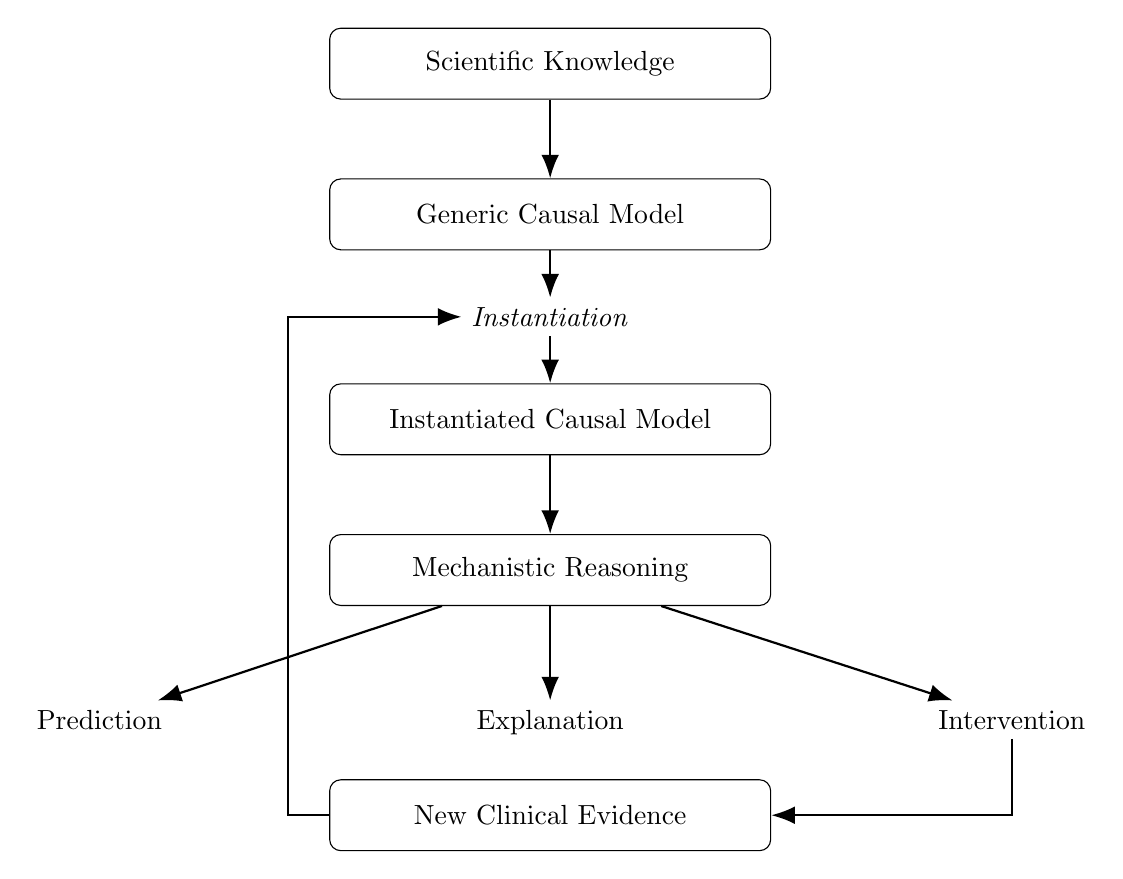
\begin{tikzpicture}[
    node distance=1.0cm,
    every node/.style={align=center},
    box/.style={
        draw,
        rounded corners,
        minimum width=5.6cm,
        minimum height=0.9cm
    },
    arrow/.style={
        -{Latex[length=3mm]},
        thick
    }
]

\node[box] (science) {Scientific Knowledge};

\node[box, below=of science] (generic) {Generic Causal Model};

\node[below=0.6cm of generic] (instantiation) {\emph{Instantiation}};

\node[box, below=0.6cm of instantiation] (patient) {Instantiated Causal Model};

\node[box, below=of patient] (reasoning) {Mechanistic Reasoning};

\node[below left=1.2cm and 2.0cm of reasoning] (prediction) {Prediction};
\node[below=1.2cm of reasoning] (explanation) {Explanation};
\node[below right=1.2cm and 2.0cm of reasoning] (intervention) {Intervention};

\node[box, below=2.2cm of reasoning] (evidence) {New Clinical Evidence};

\draw[arrow] (science) -- (generic);
\draw[arrow] (generic) -- (instantiation);
\draw[arrow] (instantiation) -- (patient);
\draw[arrow] (patient) -- (reasoning);

\draw[arrow] (reasoning) -- (prediction);
\draw[arrow] (reasoning) -- (explanation);
\draw[arrow] (reasoning) -- (intervention);

\draw[arrow] (intervention) |- (evidence);

\draw[arrow]
    (evidence.west)
    -|
    ([xshift=-2.2cm]instantiation.west)
    |- (instantiation.west);

\end{tikzpicture}

\caption{Clinical reasoning proceeds through successive instantiations of a generic causal model under changing patient-specific evidence. Each instantiated causal model supports mechanistic reasoning and clinical inquiry, which generate new evidence that constrains subsequent instantiation.}
\label{fig:instantiation}

\end{figure}

This distinction reflects the focus of the present account rather than a rejection of iterative model revision. Whereas descriptions in terms of model updating emphasize changes to the clinician's current patient-specific representation, clinical instantiation emphasizes the continuing relationship between each provisional patient-specific representation and the generic scientific model from which it is derived. These perspectives will often coincide in practice, but they highlight different aspects of the same recursive process.

The resulting instantiated model is the object of provisional clinical commitment: sufficiently supported to guide action while remaining open to replacement through subsequent instantiation as new evidence emerges.

%%%%%%%%%%%%%%%%%%%%%%%%%%%%%%%%%%%%%%%%%%%%%%%%%%%%%%%%%%%%%%
\subsection{Mechanistic Reasoning}
%%%%%%%%%%%%%%%%%%%%%%%%%%%%%%%%%%%%%%%%%%%%%%%%%%%%%%%%%%%%%%

Mechanistic reasoning plays complementary roles in scientific and clinical inquiry. Within scientific investigation, it contributes to the development and refinement of generic causal models representing disease processes, causal relationships, and the anticipated effects of interventions. Within clinical inquiry, mechanistic reasoning operates over the currently instantiated causal model representing one particular patient.

This distinction is important because the same causal knowledge serves different representational functions at the two levels. In the generic model, mechanisms are represented as possibilities believed to characterize a class of systems or patients. Such possibilities may be supported by multiple forms of scientific inquiry, including anatomical, physiological, biomechanical, and experimental mechanistic research, rather than exclusively by population-level estimates of treatment effects. In the instantiated model, they are represented as hypotheses concerning the mechanisms operative in the particular patient. Clinical mechanistic reasoning concerns the organization and consequences of those hypothesized patient-specific mechanisms.

%%%%%%%%%%%%%%%%%%%%%%%%%%%%%%%%%%%%%%%%%%%%%%%%%%%%%%%%%%%%%%
\subsection{Open Questions}
%%%%%%%%%%%%%%%%%%%%%%%%%%%%%%%%%%%%%%%%%%%%%%%%%%%%%%%%%%%%%%

The formal realization of instantiation remains open. Recent computational approaches suggest at least two importantly different routes to patient-specific representation. One route constructs an individualized model primarily from personal longitudinal data. For example, \textit{ChatDiet} applies causal discovery and causal inference to N-of-1 data to construct a personal causal model \parencite{yang_chatdiet_2024}, while Yang and Rahmani construct an individualized causal graph from each user's longitudinal dietary, activity, and glucose data \parencite{yang_personalized_2025}. Schematically, such approaches may be represented as
\[
E_{p,t} \longrightarrow M_{p,t},
\]
where patient-specific evidence is used to infer a patient-specific model.

Clinical instantiation, as formulated here, identifies a different representational problem:
\[
(M,E_{p,t}) \longrightarrow M_{p,t},
\]
where a generic causal model representing current scientific knowledge and evidence concerning the particular patient jointly constrain construction of the patient-specific explanatory representation. Whether this process is best realized through Bayesian conditioning, causal discovery, probabilistic graphical model operations, model specification, linguistic reasoning, or some coordinated composition of these and other methods remains open. The present argument does not require clinical instantiation to correspond to a novel mathematical or computational primitive. Clinical instantiation identifies the potentially composite and iterative representational process that generalized causal knowledge $M$ and patient-specific evidence $E_{p,t}$ jointly constrain the construction and reconstruction of $M_{p,t}$ during clinical inquiry. Its computational realization may therefore consist entirely of a coordinated composition of already established operations.

%%%%%%%%%%%%%%%%%%%%%%%%%%%%%%%%%%%%%%%%%%%%%%%%%%%%%%%%%%%%%%%%%%%%%%%%%%%%%%
\section{Dynamic Clinical Inquiry}
%%%%%%%%%%%%%%%%%%%%%%%%%%%%%%%%%%%%%%%%%%%%%%%%%%%%%%%%%%%%%%%%%%%%%%%%%%%%%%

Clinical reasoning proceeds through successive instantiations as new evidence accumulates through inquiry and intervention. Each instantiation produces a provisional explanatory representation of the patient that may be replaced as subsequent observations alter the evidence available.

%%%%%%%%%%%%%%%%%%%%%%%%%%%%%%%%%%%%%%%%%%%%%%%%%%%%%%%%%%%%%%
\subsection{Recursive Reasoning}
%%%%%%%%%%%%%%%%%%%%%%%%%%%%%%%%%%%%%%%%%%%%%%%%%%%%%%%%%%%%%%

Clinical inquiry proceeds recursively through successive cycles of evidence acquisition, instantiation, mechanistic reasoning, intervention, and reassessment. History taking, physical examination, diagnostic testing, and prior experience provide the evidence available at a particular stage of clinical inquiry. That evidence constrains the instantiation of the generic causal model, producing the clinician's current explanatory representation of the individual patient. The instantiated representation then guides subsequent inquiry and intervention.

Intervention is itself a source of evidence. A treatment may produce the expected response, fail to produce it, or generate an unanticipated outcome. Each possibility provides additional evidence concerning the adequacy of the current instantiated causal model. Clinical reasoning is therefore not a linear sequence moving from evidence to decision. It is a recursive process in which each cycle of inquiry generates new evidence that prompts a subsequent instantiation of the generic causal model. Explanation guides action, action generates new observations, and those observations become evidence for the next instantiation \parencite{collins_dynamic_2014,collins_synthesis_2018}.

This recursive conception is consistent with broader accounts of expert judgment in complex environments, which emphasize continual adaptation to changing circumstances rather than rigid application of predetermined methods \parencite{collins_it_2022}. Experimental work in causal cognition likewise shows that learners actively select interventions while progressively refining causal representations \parencite{gong_active_2023}.

This recursive structure may be represented schematically as

\[
\text{Evidence}
\rightarrow
\text{Instantiation}
\rightarrow
\text{Mechanistic reasoning}
\rightarrow
\text{Intervention}
\rightarrow
\text{New evidence}.
\]

Clinical action therefore extends rather than terminates inquiry: treatment, monitoring, and reassessment generate observations that may alter the next instantiation.

%%%%%%%%%%%%%%%%%%%%%%%%%%%%%%%%%%%%%%%%%%%%%%%%%%%%%%%%%%%%%%
\subsection{Dynamic Models}
%%%%%%%%%%%%%%%%%%%%%%%%%%%%%%%%%%%%%%%%%%%%%%%%%%%%%%%%%%%%%%

Because both the patient and the available evidence evolve over time, instantiated causal models must be understood as temporally indexed. The explanatory representation appropriate at one stage of clinical inquiry may no longer be adequate following disease progression, treatment, recovery, or the emergence of new observations. Patient-specific reasoning therefore requires not a single instantiation but successive instantiations throughout the course of clinical inquiry.

At a conceptual level, the clinician's instantiated model at time $t$ may be represented as

\[
M_{p,t},
\]

where $p$ identifies the particular patient and $t$ identifies the current stage of clinical inquiry.

Following the acquisition of new evidence $E_{t+1}$, the generic causal model is instantiated again, producing

\[
M_{p,t+1}.
\]

This notation intentionally leaves unspecified the mathematical realization of instantiation. It indicates only that the clinician's explanatory representation is dynamic and that each representation results from instantiating the generic causal model given the evidence currently available. Whether this process is ultimately realized through Bayesian conditioning, probabilistic graphical model operations, or another formal framework remains an open question.

Dynamic clinical inquiry consists of temporally successive instantiated models rather than a single fixed patient representation. Each model is sufficient to support current reasoning and action while remaining provisional in light of future evidence.

Clinical expertise consequently requires maintaining coherent action without treating the current instantiation as final. The clinician must remain responsive to observations that warrant construction of a different patient-specific explanatory representation.

%%%%%%%%%%%%%%%%%%%%%%%%%%%%%%%%%%%%%%%%%%%%%%%%%%%%%%%%%%%%%%%%%%%%%%%%%%%%%%
%%%%%%%%%%%%%%%%%%%%%%%%%%%%%%%%%%%%%%%%%%%%%%%%%%%%%%%%%%%%%%%%%%%%%%%%%%%%%%
\section{Relationship to Existing Theories}
%%%%%%%%%%%%%%%%%%%%%%%%%%%%%%%%%%%%%%%%%%%%%%%%%%%%%%%%%%%%%%%%%%%%%%%%%%%%%%

Clinical instantiation is intended to complement rather than replace existing theories of clinical reasoning. The following distinctions locate the proposed representational problem relative to several established frameworks.

%%%%%%%%%%%%%%%%%%%%%%%%%%%%%%%%%%%%%%%%%%%%%%%%%%%%%%%%%%%%%%
\subsection{Bayesian Reasoning}
%%%%%%%%%%%%%%%%%%%%%%%%%%%%%%%%%%%%%%%%%%%%%%%%%%%%%%%%%%%%%%

Bayesian reasoning provides a normative framework for revising beliefs under uncertainty and has been widely applied in medicine and clinical decision support \parencite{quintela-del-rio_bayesian_2019,kinney_bayesian_2021,de_grooth_bayes_2024}. Bayesian conditioning may ultimately contribute to the mathematical realization of clinical instantiation. The distinction is between such inferential operations and the construction of the patient-specific representation over which they operate.

%%%%%%%%%%%%%%%%%%%%%%%%%%%%%%%%%%%%%%%%%%%%%%%%%%%%%%%%%%%%%%
\subsection{Structural Causal Models}
%%%%%%%%%%%%%%%%%%%%%%%%%%%%%%%%%%%%%%%%%%%%%%%%%%%%%%%%%%%%%%
Structural causal models provide formal tools for representing causal relationships, interventions, and counterfactuals \parencite{pearl_causality_2013}, while probabilistic graphical models provide a broader collection of operations for representation, inference, and learning \parencite{koller_probabilistic_2009}. The generic and instantiated causal models introduced here are epistemological concepts rather than formal structural causal models, although these mathematical frameworks may provide means through which they are computationally realized.

The distinction concerns the level at which the present problem arises. Structural causal methods permit causal reasoning once an appropriate model, variables, structural relationships, and relevant evidence have been specified. Clinical instantiation concerns how generalized causal knowledge and evidence concerning a particular patient jointly constrain the construction of the particularized representation to which such operations are applied. Instantiation therefore does not compete with intervention operators or counterfactual reasoning; those operations may instead occur within an instantiated patient-specific causal representation.

%%%%%%%%%%%%%%%%%%%%%%%%%%%%%%%%%%%%%%%%%%%%%%%%%%%%%%%%%%%%%%
\subsection{Clinical Reasoning}
%%%%%%%%%%%%%%%%%%%%%%%%%%%%%%%%%%%%%%%%%%%%%%%%%%%%%%%%%%%%%%

Hypothetico-deductive models describe iterative hypothesis generation and evaluation, while illness-script and expertise theories emphasize structured knowledge, pattern recognition, and efficient diagnostic reasoning \parencite{elstein_medical_1978,schmidt_cognitive_1990,norman_research_2005,feltovich_issues_1984}. These accounts address how clinicians organize and reason with patient-specific knowledge; clinical instantiation concerns the formation of the explanatory representation on which such reasoning depends.

%%%%%%%%%%%%%%%%%%%%%%%%%%%%%%%%%%%%%%%%%%%%%%%%%%%%%%%%%%%%%%
\subsection{Knowledge Representation}
%%%%%%%%%%%%%%%%%%%%%%%%%%%%%%%%%%%%%%%%%%%%%%%%%%%%%%%%%%%%%%

The framework may also be understood as a contribution to knowledge representation. Scientific knowledge is an organized explanatory structure, while clinical inquiry produces patient-specific representations from those generic resources. Research in causal cognition treats reasoning as involving the construction and revision of causal representations through active inquiry \parencite{gong_active_2023}.

%%%%%%%%%%%%%%%%%%%%%%%%%%%%%%%%%%%%%%%%%%%%%%%%%%%%%%%%%%%%%%
\subsection{Decision Making}
%%%%%%%%%%%%%%%%%%%%%%%%%%%%%%%%%%%%%%%%%%%%%%%%%%%%%%%%%%%%%%

Decision theory concerns the rational selection of actions under uncertainty given beliefs about the current state and preferences over possible outcomes. Clinical instantiation addresses the formation of the patient-specific explanatory representation from which such decisions are made.

%%%%%%%%%%%%%%%%%%%%%%%%%%%%%%%%%%%%%%%%%%%%%%%%%%%%%%%%%%%%%%%%%%%
\section{A Computational Specification of Clinical Instantiation}
%%%%%%%%%%%%%%%%%%%%%%%%%%%%%%%%%%%%%%%%%%%%%%%%%%%%%%%%%%%%%%%%%%%

Let $M$ denote a generic causal model representing current scientific knowledge, and let $M_{p,t}$ denote the instantiated causal model representing the clinician's current explanatory understanding of patient $p$ at time $t$. Clinical instantiation may be represented abstractly as

\[
\mathcal{I}(M,E_t)=M_{p,t},
\]

where $E_t$ denotes the patient-specific evidence available at time $t$. This expression does not specify a single mathematical operation or computational primitive. Rather, $\mathcal{I}$ denotes the potentially composite and iterative process through which a patient-specific explanatory model is constructed from a generic causal model under the constraints imposed by current patient-specific evidence. The notation specifies the representational task rather than the particular sequence of inferential, representational, linguistic, or computational operations through which that task is realized.

The operator $\mathcal{I}$ is therefore conceptually distinct from an intervention operator such as Pearl's $do(\cdot)$: instantiation specifies the construction of the patient-specific representation, whereas an intervention operator supports causal reasoning within a causal model once that representation has been specified.

As new evidence becomes available, the process recurs:

\[
(M,E_t)
\xrightarrow{\mathcal{I}}
M_{p,t}
\xrightarrow{\text{reasoning/intervention}}
E_{t+1}
\xrightarrow{\mathcal{I}}
M_{p,t+1}.
\]

From a computational perspective, the problem is construction of the patient-specific representation itself. Existing probabilistic graphical model frameworks provide potentially relevant operations, including evidence conditioning, factor reduction, variable elimination, and query-specific transformations of graphical models \parencite{koller_probabilistic_2009,pearl_causality_2013}. Clinical instantiation may emerge from a coordinated composition of existing representational and inferential operations together with procedures for constructing patient-specific explanatory structure.

Recent computational approaches illustrate partial realizations of this broader task. Personalized health systems have constructed individualized statistical representations from wearable data \parencite{fang_physiollm_2024}, patient similarity graphs enriched by feature-importance models \parencite{subramanian_graph-augmented_2024}, and patient-specific causal graphs inferred from longitudinal observations \parencite{yang_chatdiet_2024,yang_personalized_2025}. Other work demonstrates how large language models can reason over an externally specified graph once such a representation is available \parencite{luo_reasoning_2024}. These approaches illustrate the growing use of explicit individualized representations while leaving open the particular transformation specified here: constructing $M_{p,t}$ from the joint constraints of a generic causal model $M$ and patient-specific evidence $E_t$.

%%%%%%%%%%%%%%%%%%%%%%%%%%%%%%%%%%%%%%%%%%%%%%%%%%%%%%%%%%%%%%
\section{Implications}
%%%%%%%%%%%%%%%%%%%%%%%%%%%%%%%%%%%%%%%%%%%%%%%%%%%%%%%%%%%%%%

%%%%%%%%%%%%%%%%%%%%%%%%%%%%%%%%%%%%%%%%%%%%%%%%%%%%%%%%%%%%%%
\subsection{Clinical Practice}
%%%%%%%%%%%%%%%%%%%%%%%%%%%%%%%%%%%%%%%%%%%%%%%%%%%%%%%%%%%%%%

Viewing clinical reasoning through clinical instantiation clarifies the relationship between scientific evidence and clinical judgment. Scientific evidence constrains the range of plausible explanatory mechanisms and interventions but does not uniquely determine the explanatory representation appropriate for an individual patient. Clinical judgment therefore includes determining which scientifically plausible mechanisms are operative in the particular case.

This perspective also provides a natural account of why experienced clinicians frequently disagree while remaining scientifically defensible. Different clinicians may instantiate different explanatory representations from the same body of scientific knowledge because they attend to different observations, assign different significance to available evidence, or anticipate different causal relationships. Such disagreement need not imply irrationality or rejection of scientific evidence. Instead, it reflects the uncertainty inherent in constructing and reasoning over provisional patient-specific explanatory representations.

%%%%%%%%%%%%%%%%%%%%%%%%%%%%%%%%%%%%%%%%%%%%%%%%%%%%%%%%%%%%%%
\subsection{Clinical Education}
%%%%%%%%%%%%%%%%%%%%%%%%%%%%%%%%%%%%%%%%%%%%%%%%%%%%%%%%%%%%%%

Clinical education has traditionally emphasized knowledge acquisition, diagnostic reasoning, and decision making. I suggest that equal attention should be given to the representational transition linking these domains. Students must learn scientific knowledge and diagnostic algorithms but also how to construct, evaluate, and reconstruct patient-specific explanatory representations as new evidence emerges through clinical inquiry. Clinical reasoning therefore becomes the application of knowledge and the progressive construction of explanatory representations appropriate for individual patients.

Expert clinicians may differ from novices not only in the extent of their knowledge or efficiency of pattern recognition, but also in their ability to construct appropriate patient-specific explanatory representations from the available scientific knowledge and clinical evidence. This interpretation is consistent with descriptions of expert physical therapist practice emphasizing contextual integration, adaptive reasoning, and individualized understanding \parencite{jensen_expertise_2007}. Expertise likewise involves greater facility in constructing, evaluating, and revising explanatory representations, maintaining provisional commitment to those representations while uncertainty persists, and recognizing when newly acquired evidence warrants another instantiation. This conception aligns naturally with contemporary views of expertise emphasizing adaptive reasoning rather than rigid application of rules \parencite{schmidt_cognitive_1990,norman_research_2005}.

%%%%%%%%%%%%%%%%%%%%%%%%%%%%%%%%%%%%%%%%%%%%%%%%%%%%%%%%%%%%%%
\subsection{Personalized Medicine}
%%%%%%%%%%%%%%%%%%%%%%%%%%%%%%%%%%%%%%%%%%%%%%%%%%%%%%%%%%%%%%

Personalized medicine has often been understood as the incorporation of increasingly individualized sources of biological and clinical information into therapeutic decision making. Advances in genomics, biomarker discovery, imaging, digital health technologies, and precision diagnostics have greatly expanded the quantity and specificity of information available about individual patients. These developments promise to improve the tailoring of interventions to individual characteristics, yet they do not by themselves explain how such information becomes reasoning about a particular patient.

Personalized health systems transform individual data into explicit patient-specific representations, including statistical summaries and correlations \parencite{fang_physiollm_2024}, similarity-based graphs \parencite{subramanian_graph-augmented_2024}, and individualized causal graphs derived from longitudinal observations \parencite{yang_chatdiet_2024,yang_personalized_2025}. These approaches suggest that personalization involves more than acquiring increasingly specific data about an individual; it also requires constructing a representation through which those data can support reasoning.

Clinical instantiation identifies a further representational problem. A patient-specific model inferred primarily from an individual's own data is not identical to a patient-specific model constructed from both generalized scientific knowledge and evidence concerning that patient. From this perspective, personalization is the construction of an individualized explanatory representation constrained by both scientific knowledge and the particular patient's presentation.

Viewed in this way, personalized medicine and evidence-based medicine need not represent competing approaches to clinical practice. Evidence-based medicine develops and refines the generic scientific representations upon which clinical reasoning depends, whereas personalized medicine concerns the construction of patient-specific explanatory representations appropriate for individual patients. Clinical instantiation provides a conceptual framework linking these complementary aims.

%%%%%%%%%%%%%%%%%%%%%%%%%%%%%%%%%%%%%%%%%%%%%%%%%%%%%%%%%%%%%%
\subsection{Artificial Intelligence}
%%%%%%%%%%%%%%%%%%%%%%%%%%%%%%%%%%%%%%%%%%%%%%%%%%%%%%%%%%%%%%

Contemporary artificial intelligence increasingly incorporates explicit individualized representations into health reasoning systems. These include patient-specific statistical representations derived from wearable data \parencite{fang_physiollm_2024}, graph-based representations of patient similarity \parencite{subramanian_graph-augmented_2024}, individualized causal models constructed from longitudinal data \parencite{yang_chatdiet_2024,yang_personalized_2025}, and methods enabling large language models to reason over externally specified graphs \parencite{luo_reasoning_2024}.

For intelligent clinical systems, the implication is that personalization should be treated as a problem of knowledge representation as well as prediction or inference. Computational architectures should distinguish the representation of generalized scientific knowledge from the construction and subsequent use of patient-specific explanatory models.

%%%%%%%%%%%%%%%%%%%%%%%%%%%%%%%%%%%%%%%%%%%%%%%%%%%%%%%%%%%%%%%%%%%%%%%%%%%%%%
\section{Conclusion}
%%%%%%%%%%%%%%%%%%%%%%%%%%%%%%%%%%%%%%%%%%%%%%%%%%%%%%%%%%%%%%%%%%%%%%%%%%%%%%

Clinical reasoning requires more than inference from scientific knowledge or observation of an individual patient. It depends upon the construction of a patient-specific explanatory representation capable of supporting reasoning and action. This paper has referred to the representational transformation by which generic scientific knowledge and patient-specific evidence jointly give rise to such a representation as \emph{clinical instantiation}.

The distinction is representational rather than competitive with existing theories of clinical reasoning. Bayesian inference, structural causal models, illness-script theory, decision theory, causal discovery, and related approaches may contribute to the construction, revision, or use of patient-specific models. Clinical instantiation identifies the representational problem that connects generalized scientific knowledge with the explanatory model of a particular patient.

Clinical reasoning can therefore be understood partly as a problem of knowledge representation. Scientific inquiry develops generic explanatory representations; clinical inquiry constructs provisional representations of particular patients from those resources as evidence accumulates. Making this transition explicit provides a conceptual basis for further work in patient-specific causal modeling, computational clinical reasoning, and intelligent clinical systems.

%%%%%%%%%%%%%%%%%%%%%%%%%%%%%%%%%%%%%%%%%%%%%%%%%%%%%%%%%%%%%%%%%%%%%%%%%%%%%%
\section*{Acknowledgments}
%%%%%%%%%%%%%%%%%%%%%%%%%%%%%%%%%%%%%%%%%%%%%%%%%%%%%%%%%%%%%%%%%%%%%%%%%%%%%%

I would like to thank XXXXX at the XXXXX for his reflections during his course on epidemiology and biostatistics in 1997 concerning the limitations of applying epidemiologic findings directly to individual patients. Although offered in the context of teaching evidence-based inference, that observation prompted questions regarding the relationship between scientific knowledge and reasoning about individual patients that ultimately motivated the ideas developed in this paper.

I also acknowledge my colleagues in the XXXXXX over many years whose discussions concerning clinical inquiry, causal reasoning, expertise, and evidence have contributed to the development of these ideas. Any errors or shortcomings remain my own.
%%%%%%%%%%%%%%%%%%%%%%%%%%%%%%%%%%%%%%%%%%%%%%%%%%%%%%%%%%%%%%%%%%%%%%%%%%%%%%
%% References
%%%%%%%%%%%%%%%%%%%%%%%%%%%%%%%%%%%%%%%%%%%%%%%%%%%%%%%%%%%%%%%%%%%%%%%%%%%%%%
\newpage
\printbibliography

\end{document}